\chapter{Ve{\'i}culos Aut{\^o}nomos}

Veículos autônomos podem ser definidos como transportes terrestres capazes de
se movimentarem de um ponto a outro por conta própria de maneira a não
necessitarem de um condutor para tomada de decisões. Esses podem ser divididos
em duas categorias: internos e externos, com os internos focando em aplicações
industriais e os externos para ambientes urbanos e consumidores finais.

Segundo \citeonline{sae2018} Existem níveis de automação veicular divididos em
5 categorias, que possuem o intuito de facilitar o entendimento da função do
veículo no ambiente para qual foi desenvolvido. Esses niveis s{\~a}o:

\begin{quote}
\begin{enumerate}
        \setcounter{enumi}{-1} 
        \item N{\~a}o automa{\c c}{\~a}o: Autonomia zero; O motorista realiza
                todas as tarefas;
        \item Dire{\c c}{\~a}o Assistida: O ve{\'i}culo {\'e} controlado pelo
                motorista mas algumas assist{\^e}ncias {\`a} condu{\c c}{\~a}o
                podem ser inclu{\'i}das no ve{\'i}culo;
        \item Automação Parcial: O veículo possui algumas funcões automatizadas
                de controle de maneira combinada, como aceleração e direção,
                mas o motorista precisa permanecer preparado para tomar o
                controle e monitorar o ambiente o tempo todo;
        \item Automação Condicional: O veículo é capaz de realizar as tarefas
                de direção sozinho em certas circunstancias, porém o motorista
                precisa permanecer preparado o tempo todo;
        \item Automação Elevada: O veículo {\'e} capaz de realizar as tarefas
                de direção sozinho em certas circunstancias. O motorista pode
                ter a opção de controlar o veículo;
        \item Automação Completa: O veículo é capaz de realizar as tarefas de
                direção sozinho sob qualquer circunstancia.  O motorista pode
                ter a opção de controlar o veículo.
\end{enumerate}
\end{quote}

\section{Ve{\'i}culo Guiado Automaticamente}

Com o avanço tecnológico estando presente em todas as frentes da economia
global atual, não há outra alternativa para fábricas dos mais diversos setores
a não ser se manter atualizadas a estas tendências, considerando que se desejam
manter relevantes no mercado. O fenômeno que mais vem se alastrando neste
ambiente no passado recente é o da Indústria 4.0, o qual define o uso de
diversas tecnologias na área de inteligência artificial, computação em nuvem,
big data e internet das coisas a fim de se automatizar processos que viriam a
demandar recursos da empresa, e consequentemente, afetando sua produtividade.
A \autoref{fig_growth} ilustra o avan{\c c}o dos investimentos na {\'a}rea ao longo
dos {\'u}ltimos anos.

\begin{figure}[htb]
        \centering
        \caption{\label{fig_growth}Gr{\'a}fico de evolu{\c c}{\~a}o de investimentos em rob{\^o}s industriais.}
        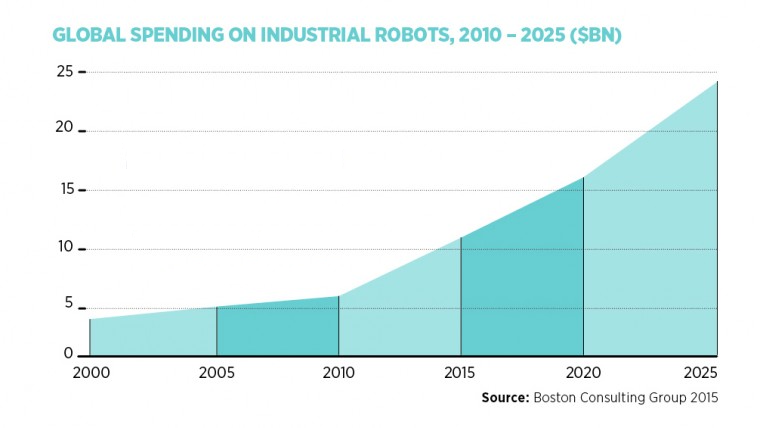
\includegraphics[width=0.7\textwidth]{images/Global-spending-industrial-robots-760x428.png}
        \legend{
                \protect\footnotemark
                Dispon{\'i}vel em: \url{https://www.raconteur.net}. Acesso em: 3 Mai. 2022.
        }
\end{figure}

\footnotetext{Imagem retirada de: \url{https://www.raconteur.net/industry-4-0-smart-machines-are-new-industrial-revolution/}}

A automação de máquinas visa permitir que os operários da produção sejam
capazes de as programar e deixar a executar funções sozinhas, com ou sem uma
supervisão externa, mas sempre sem a necessidade de um operador humano, o
avanço da quarta revolução industrial vem permitindo que estas máquinas
executem suas funções de forma mais rápida e precisa com o passar do tempo. Uma
função básica e de extrema importância para o ambiente industrial, é a de
manuseio e movimentação de materiais pela planta da fábrica, principalmente no
transporte de carga. 

Os veículos guiados automaticamente, conhecidos como AGVs, são veículos móveis
e programáveis que cumprem a função de transporte de carga dentro de um espaço
de linha de produção. Para serem de fato automatizados, devem possuir algum
meio de seleção de trajetória da qual não necessitem de intervenção manual,
assim sendo capazes de cumprir suas funções com um baixo custo operacional
\cite{kumar2016}. Estes devem ser adaptados ao ambiente em que serão
aplicados, como a inclusão de sensores necessários ou capacidade para carga a
ser carregada.

\subsection{Tipos de AGVs}

Antes de aplicar um veículo guiado automaticamente na linha de produção, se faz
necessário entender qual o problema que ele visa solucionar, existe uma série
de veículos desde os de uso geral até mais específicos, dentre os mais
popularmente conhecidos é possível citar:

\begin{itemize}
        \item \textit{Under Ride}, também chamados de \textit{Automated Guided Carts}, são carros
                que carregam plataformas móveis e se encaixam por baixo da
                carga, sendo geralmente um dos modelos mais baratos e fáceis de
                se aplicar a linha de montagem;

        \item \textit{Tugger AVG}, traduzidos como AGV Rebocador, são os veículos que
                acoplam suas cargas como um comboio e tem como principal
                vantagem a quantidade de peso elevada que conseguem puxar;

        \item \textit{Pallet Mover AVG}, ou AGV Empilhadeira é aquele que, assim como
                empilhadeiras convencionais, conseguem movimentar \textit{pallets} e
                bobinas das linhas de produção até armazéns, podendo levantar
                sua carga de acordo com a altura máxima do equipamento;

        \item \textit{Unit Load AVG}, traduzidos como AVG com Mesa de Transferência, são
                capazes de transferir uma carga que carregam sobre eles para
                outras plataformas através de um sistema de esteira rolantes
                que possuem.

\end{itemize}

Além dos citados, existem outros tipos de modelos empregados na indústria que
podem vir a ser utilizados por empresas em situações específicas de sua
necessidade, adaptando os AGVs de acordo com sua linha de produção. É possível
verificar alguns exemplos na \autoref{fig_agv}.

\begin{figure}[htb]
        \centering
        \caption{\label{fig_agv}Modelos diversos de AGVs adaptados para suas aplica{\c c}{\~o}es.}
        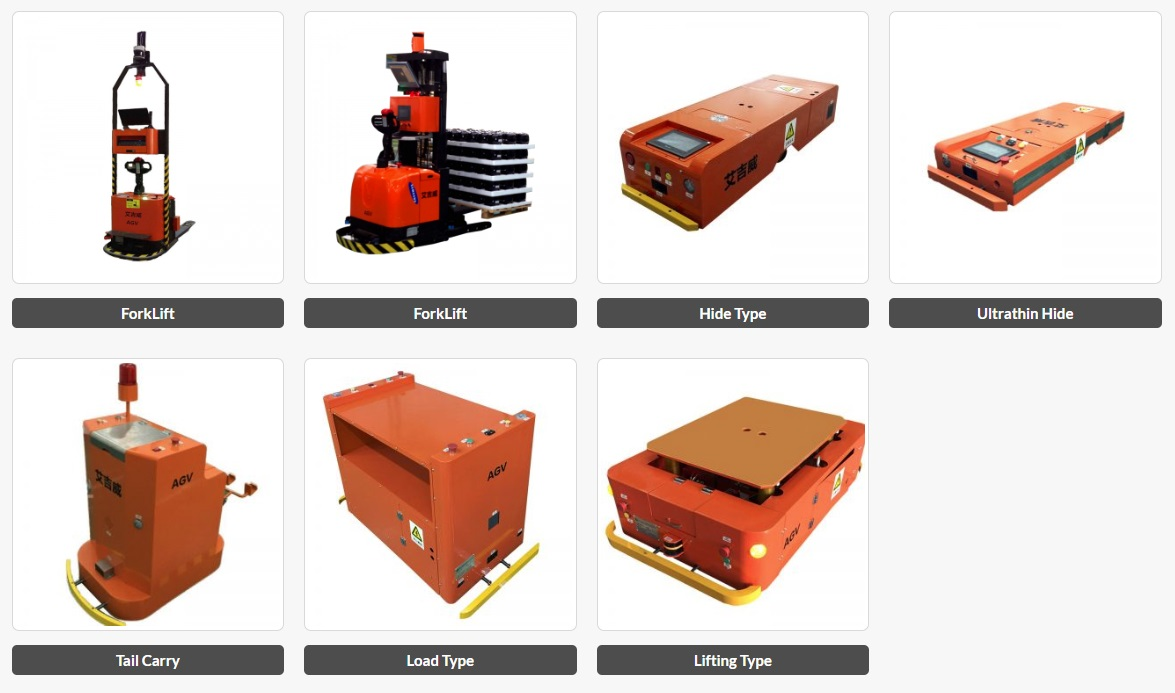
\includegraphics[width=0.7\textwidth]{images/suzhou-agv-robot-products.jpg}
        \legend{
                \protect\footnotemark
                Dispon{\'i}vel em: \url{https://www.agvnetwork.com}. Acesso em: 3 Mai. 2022.
        }
\end{figure}

\footnotetext{Imagem retirada de: \url{https://www.agvnetwork.com/automated-guided-vehicles-manufacturers}}

\subsection{M{\'e}todos de navega{\c c}{\~a}o de AGVs}

Existem diversas técnicas aplicáveis a fim de se obter uma navegação
automatizada dos AVGs, metodologias mais antigas se baseiam em sensoriamento
indutivo, ótico ou magnético e soluções mais modernas empregam o uso de visão
computacional e GPS, a melhor solução é encontrada justamente na mais bem
aplicável ao problema proposto.

\begin{itemize}

        \item Navegação de caminho físico exige que, de certa forma, o AVG seja
                capaz de seguir um trajeto definido na superfície de movimento
                e caminhe por ele até ser necessário tomar alguma ação
                baseando-se em seu algoritmo, mesmo sem saber onde exatamente
                ele se localiza geograficamente. Esta movimentação pode ocorrer
                graças a diferentes tipos de sensoriamento:

        \begin{itemize}
                \item Ótico: navegação baseada em sensores que identificam uma
                        fita que contraste em cor com o restante do chão da
                        fábrica, permitindo que o AVG se movimente enquanto a
                        guia estiver presente e a seguindo, ajustando sua rota
                        quando necessário, esta checagem de trajeto também pode
                        ser feita através de códigos QR presentes no chão;

                \item Indutivo: navegação baseada em sensores indutivos
                        instalados no AVG que se mantém em movimento enquanto
                        estiver no alcance de fitas magnéticas sobre ou sob o
                        chão da fábrica, ajustando seu trajeto por onde a fita
                        o guiar.

        \end{itemize}

        \item Navegação de caminho virtual é onde o mapa do trajeto aplicável
                ao AGV está presente dentro de sua memória ou em um computador
                central (transmitido pela rede), de modo que a navegação se
                torne mais facilmente adaptável, em contrapartida, se faz
                necessário saber a posição do veículo para que o mesmo possa
                interpretar o melhor trajeto a se percorrer. Esta movimentação
                também possui algumas variações de navegação sujeitas a
                implementação:

        \begin{itemize}

                \item Laser: raios são emitidos partindo do AGV e com base na
                        resposta de refletores montados ao seu redor na
                        fábrica, ele consegue identificar suas coordenadas e se
                        basear nelas para encontrar sua rota. Existem exemplos
                        de sensores que conseguem captar respostas do ambiente
                        sem a necessidade de refletores instalados;

                \item GPS: estes AGVs possuem receptores GPS que captam o sinal
                        de satélites e assim se identificam no plano, este
                        sendo um método custoso por exigir uma série de sinais
                        externos, geralmente possui sua lógica empregada com
                        radares locais;

                \item Guiada por visão: através de uma câmera, o veículo
                        consegue interpretar os objetos a sua frente como uma
                        projeção 2D e se localizar no espaço.

        \end{itemize}

\end{itemize}

Estes veículos que não necessitam de guias externos também são chamados de AMR,
que diferentemente dos AGVs convencionais, possuem inteligência própria e
geralmente se encontram atrelados a contextos de Indústria 4.0 e Internet das
Coisas. Novamente, a melhor solução para cada problema depende de sua
aplicação, a navegação por caminho física é mais fácil de ser implementada e já
pode ser encontrada na indústria a muito tempo enquanto a por caminho virtual
exige uma complexidade de mapeamento prévio mas a torna mais versátil.

%É possível verificar na \autoref{fig_amr} diferentes tipos de tecnologias de
%navegação para AVGs, cada um com o ambiente adaptado a sua aplicação.
%
%\begin{figure}[htb]
%        \centering
%        \caption{\label{fig_amr}Tecnologias de Navegação de AGVs.}
%        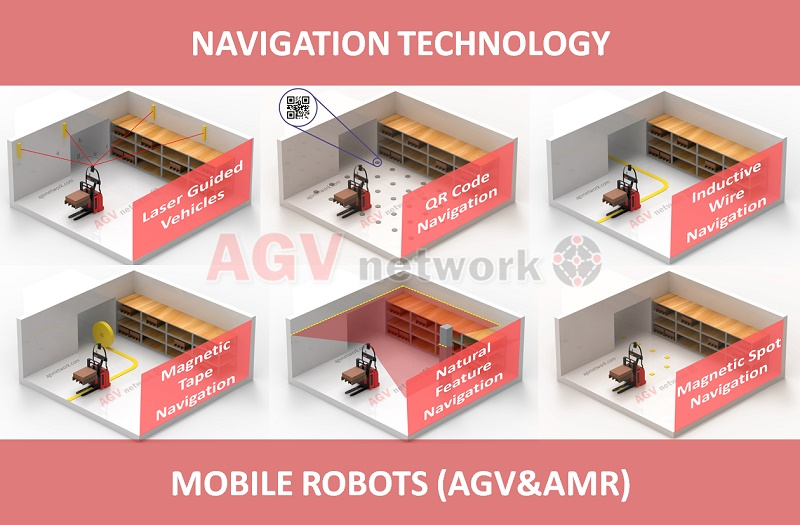
\includegraphics[width=0.7\textwidth]{images/AGV_and_AMR_Navigation_Technology.jpg}
%        \legend{
%                \protect\footnotemark
%                Dispon{\'i}vel em: \url{https://www.agvnetwork.com}. Acesso em: 3 Mai. 2022.
%        }
%\end{figure}

%\footnotetext{Imagem retirada de: \url{https://www.agvnetwork.com/types-of-automated-guided-vehicles}}

\section{Carros Aut{\^o}nomos}

Veículos de condução autônoma externa são caracterizados pela capacidade de se
movimentar em ambientes não controlados, no contexto urbano, sem a necessidade
e interferência de um condutor de maneira direta \cite{usp2016}. A tecnologia
embarcada nesses veículos possui mais de trinta anos, porém, somente no começo
do século XXI começou a ser difundida entre o grande público e se tornar mais
popular.

\subsection{Hist{\'o}ria}

Sabe-se que estudos envolvendo um veículo terrestre capaz de se locomover sem a
necessidade de um motorista é datado de 1920, onde engenheiros e pesquisadores
de Ohio, nos Estados Unidos, desenvolveram um veículo de pequeno porte, incapaz
de transportar passageiros, que possuía capacidade de receber instruções via
rádio e realizar comandos de atuação nos sistemas de direção do veículo,
eliminando a necessidade de um condutor.  A limitação desse sistema estava no
\textit{hardware}, incapaz de tomar decisões e necessitando de instruções externas para
guiá-lo. Apesar de simples, esse foi o início da busca de um veículo capaz de
se autoconduzir. 

Em 1950, sensores capazes de detectar velocidade e localização dos veículos
foram utilizados em estradas de teste para captar e enviar informações via
rádio para os carros equipados com receptores, sendo o precursor o modelo GM
Firebird II em 1956. Porém, tal ideia foi descontinuada pela complexidade de
instalação dos sensores nas estradas, assim como o gerenciamento de um tráfego
constante e composto por veículos não equipados com a tecnologia. Mesmo com o
insucesso da solução, já havia avanço quando comparado com o modelo via rádio,
com o sistema possuindo um \textit{software} capaz de tomar decisões como acelerar e
frear sem interferência externa.

Com o avanço da computação e do processamento de dados, foi possível
desenvolver um veículo equipado com diferentes tipos de sensores, processadores
e câmeras capazes de identificar, por exemplo, um carro à frente e evitar
colisões descartando informações externas, sendo a decisão tomada pelo próprio
sistema presente no veículo. Com isso, o primeiro carro realmente autônomo da
história foi o NavLab 1, lançado em 1986 \cite{estadao2020}, demonstrado na \autoref{fig_navlab}. 

\begin{figure}[htb]
        \centering
        \caption{\label{fig_navlab}NavLab 1.}
        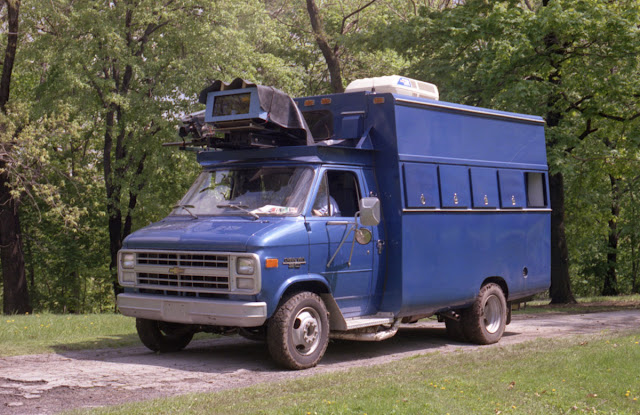
\includegraphics[width=0.5\textwidth]{images/EG-navlab1-CMU-media-relations.jpg}
        \legend{
                \protect\footnotemark
                Dispon{\'i}vel em: \url{https://www.rediscoverthe80s.com}. Acesso em: 3 Mai. 2022.
        }
\end{figure}
\footnotetext{Imagem retirada de: \url{https://www.rediscoverthe80s.com/2016/11/navlab-the-selfdriving-car-of-the-80s.html}}

\subsection{Ve{\'i}culos aut{\^o}nomos atuais}

Mesmo com os conceitos de funcionamento de um veículo autônomo sendo definido
em 1980 e o poder computacional dos dispositivos avançarem ano após ano, tal
tecnologia permaneceu distante do consumidor final por um longo período de
tempo dada sua complexidade de navegação em situações urbanas do cotidiano. 

Segundo \citeonline{townsend2020}, somente em 2009 empresas, como o Google, iniciaram
pesquisas com o intuito de atingir um veículo autônomo urbano. Empresas líderes
de mercado como Ford, Mercedes-Benz, Volkswagen e BMW, por exemplo, começaram a
desenvolver veículos capazes de dirigir sozinhos. No decorrer do
desenvolvimento, tecnologias criadas para os futuros autônomos foram sendo
implementadas aos poucos em veículos comerciais, aumentando o nível dos mesmos
na escala de automação veicular.

Os veículos começaram no nível 0, possuindo tecnologias como frenagem
automática de emergência, detecção de ponto cego e aviso de evasão de faixa,
por exemplo, aumentando a complexidade conforme o desenvolvimento aumentava,
até chegarem ao nível 1, com correção automática em caso de evasão de faixa e
controle de cruzeiro adaptativo, por exemplo.

Porém, somente com o avanço dos carros elétricos, em específico pela marca
Tesla, veículos de nível 2 e 3 chegaram ao consumidor final e começaram a se
popularizar.

\subsubsection{Tesla}

A Tesla foi criada em 2003 com o intuito de desenvolver bons carros elétricos,
capazes de competir diretamente com os a combustão, e, dessa forma, os
popularizar.  Os carros se tornaram populares entre os entusiastas,
consolidando a empresa, mas ainda sim eram considerados de nicho, possuindo um
alto valor de produção e não conseguindo atrair a curiosidade e o interesse do
grande público.

Em 2015 a Tesla lança seu sistema nível 2 de automação veicular, chamado de
Tesla \textit{Autopilot}, para todos os proprietários do modelo \textit{Model
S}, demonstrado na \autoref{fig_models}. O \textit{Autopilot} é capaz de levar
o veículo do ponto A ao ponto B, com uma rota traçada anteriormente pelo GPS,
de maneira em que o condutor não precise conduzir o veículo durante o percurso. 

O Autopilot surgiu como um grande avanço na trajetória ao nível de 5 de
automação veicular, sendo usado também como peça publicitária para chamar a
atenção do público os veículos elétricos, conseguindo os popularizar. Além
disso, chamou também a atenção da indústria automotiva de modo geral,
acelerando as montadoras tradicionais de veículos a combustão, dada a cobrança
e interesse do consumidor final, em seu desenvolvimento de uma tecnologia de
automação similar a da Tesla capaz de atingir o  nível 2 ou nível 3.

\begin{figure}[htb]
        \centering
        \caption{\label{fig_models}Tesla Model S.}
        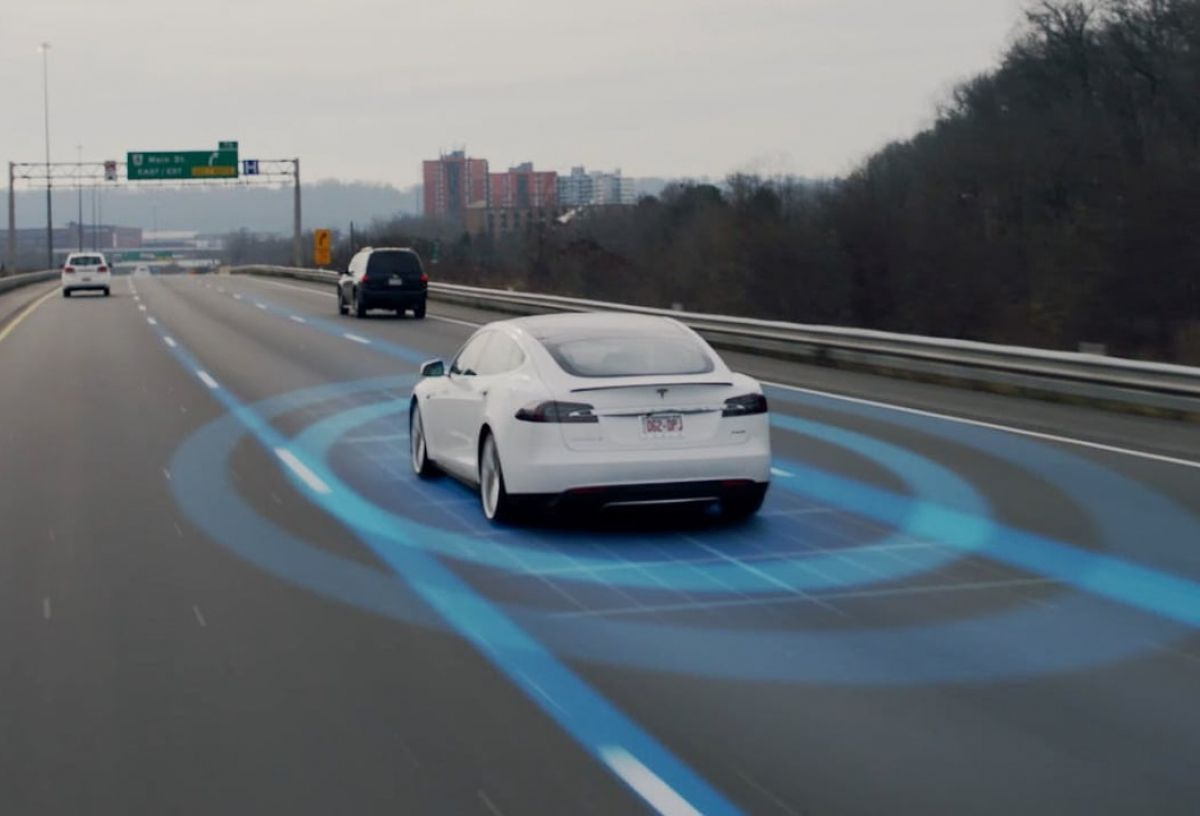
\includegraphics[width=0.7\textwidth]{images/01e87df6ce89a7b3ea1141da979d599b.jpg}
        \legend{
                \protect\footnotemark
                Dispon{\'i}vel em: \url{https://www.tesla.com/videos/enhance-your-commute-autopilot}. Acesso em: 3 Mai. 2022.
        }
\end{figure}

\footnotetext{Imagem retirada de: \url{https://www.tesla.com/videos/enhance-your-commute-autopilot}}

Para seu funcionamento, o Autopilot utiliza um \textit{hardware} similar ao NavLab 1,
com câmeras 360, sensores ultra-sônicos, sensores infravermelho e uma vasta
gama de processadores com propósitos variados. Controlando todo o complexo
equipamento presente fisicamente, existe o \textit{software} utilizando o método de
visão computacional.

\subsubsection{Vis{\~a}o Computacional}

Visão computacional é um área da inteligência artificial que permite
computadores e sistemas digitais abstrair informações de imagens, vídeos,
sensores diversos e qualquer outra entrada digital para tomar ações e decisões
baseadas nos dados adquiridos nas entradas \cite{ibm2019}.  

Para tal é necessário uma alta quantidade de dados, onde, computacionalmente,
seja possível treinar o modelo desenvolvido e interpretar de maneira correta as
entradas. Para treinar um modelo capaz de identificar um pneu, por exemplo, é
necessário munir as entradas com diversas imagens de pneus em diferentes
situações para que seja possível observar um padrão, e, dessa forma, o modelo
caracterizá-lo como um pneu.

Duas tecnologias essenciais para o desenvolvimento de um modelo que utiliza
visão computacional são: uma divisão do \textit{Machine Learning} chamado
\textit{Deep Learning} em conjunto com uma Rede Neural Convolucional.

O \textit{deep learning} utiliza modelos de algoritmos capazes de gerar os
padrões, capacitando o modelo a distinguir uma coisa da outra. Para isso
utiliza as imagens de treinamento e as difere uma das outras, observando as
diferenças gerando categorias para cada imagem e aprendendo com essas mesmas
categorias.

Já a Rede Neural Convolucional, auxilia o \textit{deep learning} nessa tarefa
de auto aprendizado, quebrando as imagens em pixels e as categorizando por
distância, discernindo bordas e formas, gerando, com esses pixels analisados,
tags e rótulos. Essas demarcações são utilizadas para gerar convoluções,
operação matemática capaz de gerar um terceira função a partir de outras duas
funções, predizendo o que está sendo observado. A rede neural roda então uma
série de convoluções verificando a acurácia das mesmas até que chegue ao valor
definido pelo modelo.

A visão computacional é utilizada por diversas montadoras e se prova até o
momento o método mais eficaz para veículos autônomos externos, porém, possui um
alto grau de complexidade e esbarra em diversas questões éticas e legais no que
se diz respeito à legislação de trânsito pela questão da segurança de um
veículo autônomo trafegando entres veículos não autônomos.

